%!TEX root=paper/paper.tex
\chapter{Missing value imputation}\label{sec:imputation_evaluation}

We evaluate reconstruction and classification error on two datasets: Digits and Scenes-15.
Two feature selection policies are considered: Random and Clustered.
For each policy, we consider Independent and Block-wise selection patterns.

We find that mean imputation with classifier retraining is a reasonably well-performing approach.
Nearest Neighbor methods perform best but are the most expensive.
Gaussian imputation method performs very well, but is also expensive.
Training additional classifiers for clusters of observed feature subsets did not improve performance.

Feature selection had four experimental conditions.
\begin{itemize}
\item In \textbf{Random, Independent} selection, each feature was selected independently, and the total number of possible masks for a given budget was not bounded, such that each test instance could have a unique mask (if the number of test instances $N$ was less than the total number of possible feature subsets $2^F$.
\item In \textbf{Random, Block-wise} selection, there was no bound on the number of possible masks for a given budget, but features were selected by blocks.
\item In \textbf{Clustered, Independent} selection, each feature was selected independently, but there were at most $K$ possible masks for a given budget.
\item In \textbf{Clustered, Block-wise} selection, there were at most $K$ possible masks for a budget, and features were selected by blocks.
\end{itemize}

All datasets were first standardized by subtracting the row mean and dividing by the row standard deviation.

\section{Digits}
The Digits dataset contains 8x8 grayscale images of hand-written digits 1-10.
Each of the 10 classes has 200 samples, for a total of 2000 images and 64 features.

The dataset was split 60-40 into training and testing sets.
The number of clusters for clustered selection was 10.
For block-wise feature selection, the number of blocks was set to 8.

Figure~\ref{fig:digits} shows the results; here we summarize the conclusions:

\begin{itemize}
\item Mean imputation has highest reconstruction and classification error.
\item Dot product-based kNN imputation performs worse than Gaussian imputation for both reconstruction and classification, and is slower.
\item Euclidean distance-based kNN imputation performs best, but is slowest.
\item Training additional classifiers for clusters of observed subsets slightly decreased classification error, but only if the number of clusters was high.
\item These results hold for all policy experimental conditions.
\end{itemize}

\begin{figure}[ht]
    \centering
    \begin{subfigure}[b]{.9\textwidth}
        \centering
        \includegraphics[width=\linewidth]{../../figures/281b_for_thesis/digits/random_-1/subplots.png}
        \caption{Random, independent feature selection.\vspace{.2cm}}
    \end{subfigure}
    \begin{subfigure}[b]{.9\textwidth}
        \centering
        \includegraphics[width=\linewidth]{../../figures/281b_for_thesis/digits/random_8/subplots.png}
        \caption{Random, block-wise (8 blocks) feature selection.\vspace{.2cm}}
    \end{subfigure}
    \begin{subfigure}[b]{\textwidth}
        \centering
        \includegraphics[width=\linewidth]{../../figures/281b_for_thesis/digits/clustered_-1/subplots.png}
        \caption{Clustered (10 clusters), independent feature selection.\vspace{.2cm}}
    \end{subfigure}
    \begin{subfigure}[b]{\textwidth}
        \centering
        \includegraphics[width=\linewidth]{../../figures/281b_for_thesis/digits/clustered_8/subplots.png}
        \caption{Clustered (10 clusters), block-wise (8 blocks) feature selection.\vspace{.2cm}}
    \end{subfigure}
    % \begin{subfigure}[t]{.48\textwidth}
    %     \centering
    %     \tiny{\begin{tabular}{ll}
\toprule
                                   & clustered\\
\midrule
gaussian, full                     & 0.206\\
gaussian, retrained                & 0.206\\
kNN (dot)                          & 0.241\\
kNN (dot), full                    & 0.211\\
kNN (euclidean)                    & \textbf{0.166}\\
kNN (euclidean), full              & 0.170\\
mean, full                         & 0.308\\
mean, retrained                    & 0.223\\
mean, retrained, 5 clusters        & 0.301\\
mean, retrained, all (10) clusters & 0.194\\
\bottomrule
\end{tabular}
}
    %     \caption{Areas under the Classification Error vs. Budget curves. Lower is better.}
    % \end{subfigure}\hfill%
    % \begin{subfigure}[t]{.48\textwidth}
    %     \centering
    %     \tiny{\begin{tabular}{lllll}
\toprule
                & clustered & clustered, blocks & clustered & clustered, blocks\\
\midrule
gaussian        & 94.76     & 93.16             & 151.43    & 150.06\\
kNN (dot)       & 102.5     & 97.59             & 180.11    & 170.79\\
kNN (euclidean) & 87.33     & 87.16             & 159.33    & 159.09\\
mean            & 120.08    & 114.02            & 252.38    & 237.75\\
\bottomrule
\end{tabular}

}
    %     \caption{Areas under the Reconstruction RMSE vs. Budget curves. Lower is better.}
    % \end{subfigure}
    \caption{All results on the \textbf{Digits} dataset.}
    \label{fig:digits}
\end{figure}

\section{Scenes-15}
The Scene-15 dataset \parencite{Lazebnik-CVPR-2006} contains 4485 images from 15 visual scene classes.
The task is to identify classify images according to scene.

Following \parencite{Xiao-CVPR-2010}, we extracted 14 different visual features (GIST, HOG, TinyImages, LBP, SIFT, Line Histograms, Self-Similarity, Textons, Color Histograms, and variations).
Separate multi-class linear SVMs were trained on each feature channel, using a random 100 positive example images per class for training.
We used the liblinear implementation, and cross-validated the penalty parameter $C$.

The trained SVMs were evaluated on the images not used for training, resulting in a dataset of 2238 vectors of 210 confidence values: 15 classes for each of the 14 feature channels.
This dataset was split 60-40 into training and test sets for our experiments.
The number of clusters for clustered selection was 10.
For block-wise feature selection, the number of blocks was set to 5.

Figure~\ref{fig:scenes} shows the results.
The conclusions are much the same as for the \textbf{Digits} dataset, with the following additional observations:
\begin{itemize}
\item Gaussian imputation is more costly than kNN on this data; the feature dimensions is more than twice that of the Digits data.
\item For block-wise feature selection, mean imputation with retraining is as good as any other approach, and of course by far the fastest.
\end{itemize}

\begin{figure}[ht]
    \centering
    \begin{subfigure}[b]{.8\textwidth}
        \centering
        \includegraphics[width=\linewidth]{../../figures/281b_for_thesis/scenes/random_-1/subplots.png}
        \caption{Random, independent feature selection.\vspace{.2cm}}
    \end{subfigure}
    \begin{subfigure}[b]{.8\textwidth}
        \centering
        \includegraphics[width=\linewidth]{../../figures/281b_for_thesis/scenes/random_5/subplots.png}
        \caption{Random, block-wise (8 blocks) feature selection.\vspace{.2cm}}
    \end{subfigure}
    \begin{subfigure}[b]{\textwidth}
        \centering
        \includegraphics[width=\linewidth]{../../figures/281b_for_thesis/scenes/clustered_-1/subplots.png}
        \caption{Clustered (10 clusters), independent feature selection.\vspace{.2cm}}
    \end{subfigure}
    \begin{subfigure}[b]{\textwidth}
        \centering
        \includegraphics[width=\linewidth]{../../figures/281b_for_thesis/scenes/clustered_5/subplots.png}
        \caption{Clustered (10 clusters), block-wise (8 blocks) feature selection.\vspace{.2cm}}
    \end{subfigure}
    % \begin{subfigure}[b]{1\textwidth}
    %     \centering
    %     \tiny{\begin{tabular}{ll}
\toprule
                                   & clustered\\
\midrule
gaussian, full                     & 0.206\\
gaussian, retrained                & 0.206\\
kNN (dot)                          & 0.241\\
kNN (dot), full                    & 0.211\\
kNN (euclidean)                    & \textbf{0.166}\\
kNN (euclidean), full              & 0.170\\
mean, full                         & 0.308\\
mean, retrained                    & 0.223\\
mean, retrained, 5 clusters        & 0.301\\
mean, retrained, all (10) clusters & 0.194\\
\bottomrule
\end{tabular}
}
    %     \caption{Areas under the Classification Error vs. Budget curves. Lower is better.}
    % \end{subfigure}
    % \begin{subfigure}[b]{1\textwidth}
    %     \centering
    %     \tiny{\begin{tabular}{lllll}
\toprule
                & clustered & clustered, blocks & clustered & clustered, blocks\\
\midrule
gaussian        & 94.76     & 93.16             & 151.43    & 150.06\\
kNN (dot)       & 102.5     & 97.59             & 180.11    & 170.79\\
kNN (euclidean) & 87.33     & 87.16             & 159.33    & 159.09\\
mean            & 120.08    & 114.02            & 252.38    & 237.75\\
\bottomrule
\end{tabular}

}
    %     \caption{Areas under the Reconstruction RMSE vs. Budget curves. Lower is better.}
    % \end{subfigure}
    \caption{All results on the \textbf{Scenes-15} dataset.}
    \label{fig:scenes}
\end{figure}

\section{Conclusion}

On both datasets, and for all feature selection approaches, we find that mean imputation (with a classifier trained on imputed data) is a well-performing approach.
Nearest Neighbor and Gaussian methods perform best but are the most expensive; Gaussian scales poorly with number of features, while NN scales poorly with size of training set.
Training additional classifiers for clusters of observed feature subsets also did not signficantly improve performance on these datasets.
